\section{Windows}

Officially, the pbdR team does not support gaming consoles.  However, it is possible to install pbdR packages on Windows.

\subsection{R and Rtools}

The instructions and screenshots for this document are for version 2.15.1 of R, but later versions should be very similar, if not identical.






\subsubsection{R}

\begin{enumerate}
  \item Download R: \url{http://cran.r-project.org/bin/windows/base/}
%   \begin{center}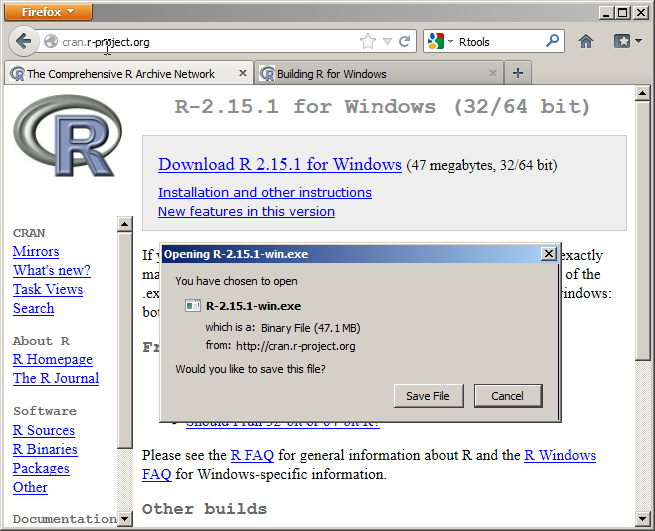
\includegraphics[scale=.5]{windows/pics/R_1} \label{enum:windl}\end{center}
  %
  \item Open the saved file from \ref{enum:windl} above to begin the installation, and click 'Next' to continue.
%   \begin{center}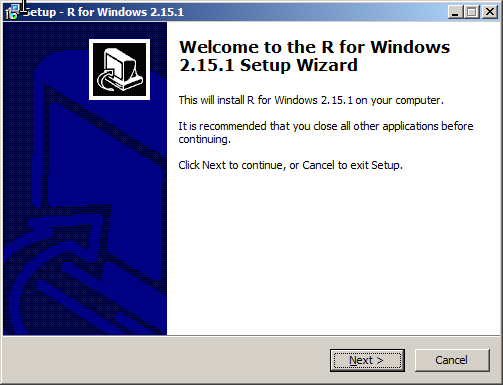
\includegraphics[scale=.65]{windows/pics/R_2} \label{enum:windl}\end{center}
  %
  \item Make sure that you agree with the License Click 'Next':
%   \begin{center}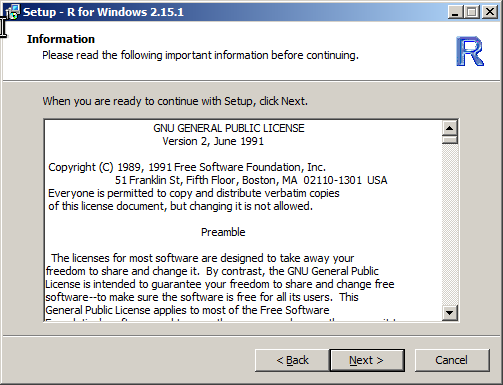
\includegraphics[scale=.65]{windows/pics/R_3} \label{enum:windl}\end{center}
  \item \code{asdf}
\end{enumerate}





\subsubsection{Rtools}


